The Camera System Layer contains a camera subsystem, gimbal subsystem, and gimbal controller subsystem. These subsystems send raw video streams to the Processing System Layer and receive head tracking angles from it.

\begin{figure}[h!]
	\centering
 	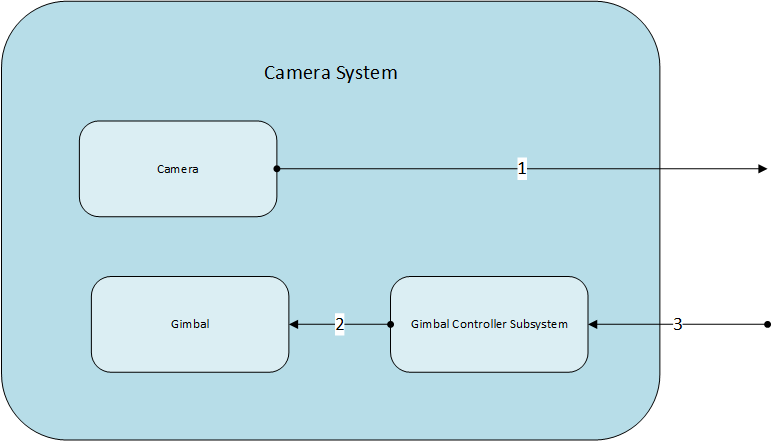
\includegraphics[width=0.75\textwidth]{images/camerasubsystem}
 \caption{Camera System Layer Subsystem Description Diagram}
\end{figure}

\subsection{Camera Subsystem}
The camera subsystem will send the raw video streams directly to the Processing System to be processed.

\subsubsection{Assumptions}
This subsystem is assumed to be handled by the firmware already built into the cameras.

\subsubsection{Responsibilities}
This subsystem is responsible for giving video input to the system that will eventually end up in the virtual reality headset the user is wearing.

\subsubsection{Subsystem Interfaces}
This subsystem will have a one-way interface which is with the Processing System's video input subsystem. Through this interface, the raw video will be streamed and processed.

\begin {table}[H]
\caption {Camera Subsystem interfaces} 
\begin{center}
    \begin{tabular}{ | p{1cm} | p{6cm} | p{3cm} | p{3cm} |}
    \hline
    ID & Description & Inputs & Outputs \\ \hline
    \#1 & Processing System - Video Input Subsystem & \pbox{3cm}{N/A} & \pbox{3cm}{Raw video footage}  \\ \hline
    \end{tabular}
\end{center}
\end{table}

\subsection{Gimbal Subsystem}
This subsystem communicates with the gimbal controller subsystem to move each gimbal motor to their position.

\subsubsection{Assumptions}
Head tracking angles are read in a certain order from the translations of angles from the gimbal controller subsystem's serial communication.

\subsubsection{Responsibilities}
This subsystem is responsible for the movement of the gimbals by reading and moving into the positions given by the gimbal controller subsystem's head tracking angles.

\subsubsection{Subsystem Interfaces}
This subsystem will have a one-way interface. Head tracking angles are received from the gimbal controller subsystem.

\begin {table}[H]
\caption {Gimbal Subsystem interfaces} 
\begin{center}
    \begin{tabular}{ | p{1cm} | p{6cm} | p{3cm} | p{3cm} |}
    \hline
    ID & Description & Inputs & Outputs \\ \hline
    \#2 & Gimbal Controller Subsystem & \pbox{3cm}{Translated head tracking angles} & \pbox{3cm}{N/A}  \\ \hline
    \end{tabular}
\end{center}
\end{table}

\subsection{Gimbal Controller Subsystem}
Head tracking data will be received and handled in this subsystem from the Processing System before sending the resulting data to the gimbal subsystem.

\subsubsection{Assumptions}
None

\subsubsection{Responsibilities}
This subsystem will receive the head tracking angles from the Processing System. It will then translate the angles to be sent to the gimbal subsystem.

\subsubsection{Subsystem Interfaces}
This subsystem will have two one-way interface. The Processing system will send the data to this subsystem which will then send it to the gimbal subsystem.

\begin {table}[H]
\caption {Gimbal Controller Subsystem interfaces} 
\begin{center}
    \begin{tabular}{ | p{1cm} | p{6cm} | p{3cm} | p{3cm} |}
    \hline
    ID & Description & Inputs & Outputs \\ \hline
    \#3 & Gimbal Subsystem & \pbox{3cm}{N/A} & \pbox{3cm}{Translated head tracking angles}  \\ \hline
     \#4 & Processing System -  Gimbal Controller Subsystem & \pbox{3cm}{Head tracking angles} & \pbox{3cm}{N/A}  \\ \hline
    \end{tabular}
\end{center}
\end{table}